
\begin{textarea}[]
	\only<1>{
		\begin{columns}[c]
			\column{.3\textwidth}
			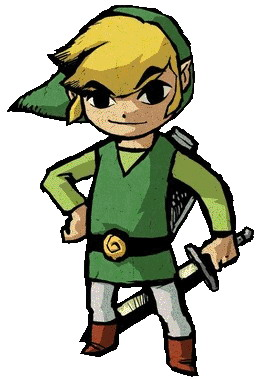
\includegraphics[height=1.0\linewidth]{categories/media/Wakerlink.jpg}
			\column{.5\textwidth}
			Often given a girls name, this little fellow is the one, actually saving the princess whose name he is called incorrectly very often.
		\end{columns}

	}
	\only<2>{
		Who is Link?
	}
\end{textarea}



\begin{textarea}[]
	\only<1>{
		Having celebrated its 20 year anniversary with a super bowl commercial, this video game series makes kids memorize the name of currently 720 characters. It started with 150.
	}
	\only<2>{
		What is Pokemon?
	}
\end{textarea}



\begin{textarea}[]
	\only<1>{
		This 2011 sandbox video game originally created by Swedish programmer Markus "Notch" Persson would probably not win an award for best graphics.

		However, this didn't stop Microsoft from buying it for US\$ 2.5 billion.
	}
	\only<2>{
		What is Minecraft?
	}
\end{textarea}

 \begin{textarea}[]
 	\only<1>{
 		With this space flight simulator, you will develop all the skill to go into space. Even NASA applauded the physical accuracy behind it.

 	}
 	\only<2>{
 		What is Kerbal Space Program?
 	}
 \end{textarea}

 \begin{textarea}[]
 	\only<1>{
   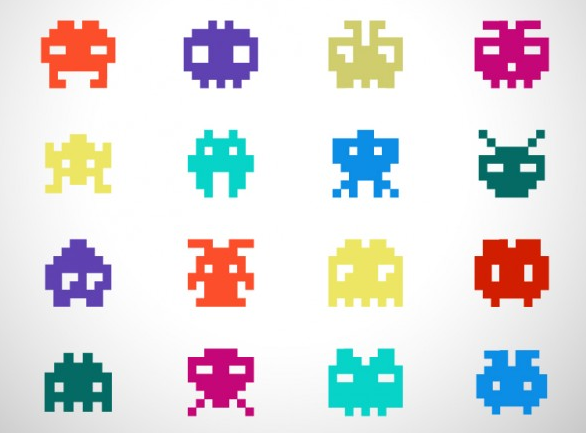
\includegraphics[width=0.5\textwidth]{categories/media/videogames/space-invaders.png}
 	}
 	\only<2>{
 		What is Space Invaders?
 	}
 \end{textarea}

 \begin{textarea}[]
 	\only<1>{
    Blinky, Pinky, Inky and Clyde roam the maze, trying to catch this yellow dot-eating fellow.
 	}
 	\only<2>{
 		What is Pac-Man?
 	}
 \end{textarea}

 \begin{textarea}[]
   \only<1>{
   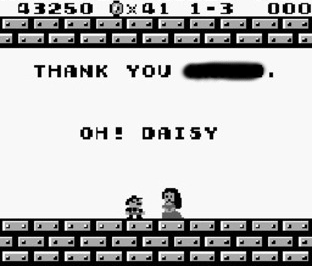
\includegraphics[width=0.5\textwidth]{categories/media/videogames/super-mario-land.png}
   }
   \only<2>{
     What is Super Mario Land?
   }
 \end{textarea}
